%------------------------------------------------------------------------------%
% APPENDICES
%------------------------------------------------------------------------------%
\appendix
% Changes the table and figure counting to A.1 style
\renewcommand\thefigure{\thechapter.\arabic{figure}}
\renewcommand\thetable{\thechapter.\arabic{table}}

%--- Appendix ---------------------------------------------------------------%

\chapter{Appendix}

\begin{figure}[h]
\captionsetup{justification=centering}
  \caption{No Stepping Stone \& Complete Information Time Series of Group Strategy}
   \label{fig:Series1C}
    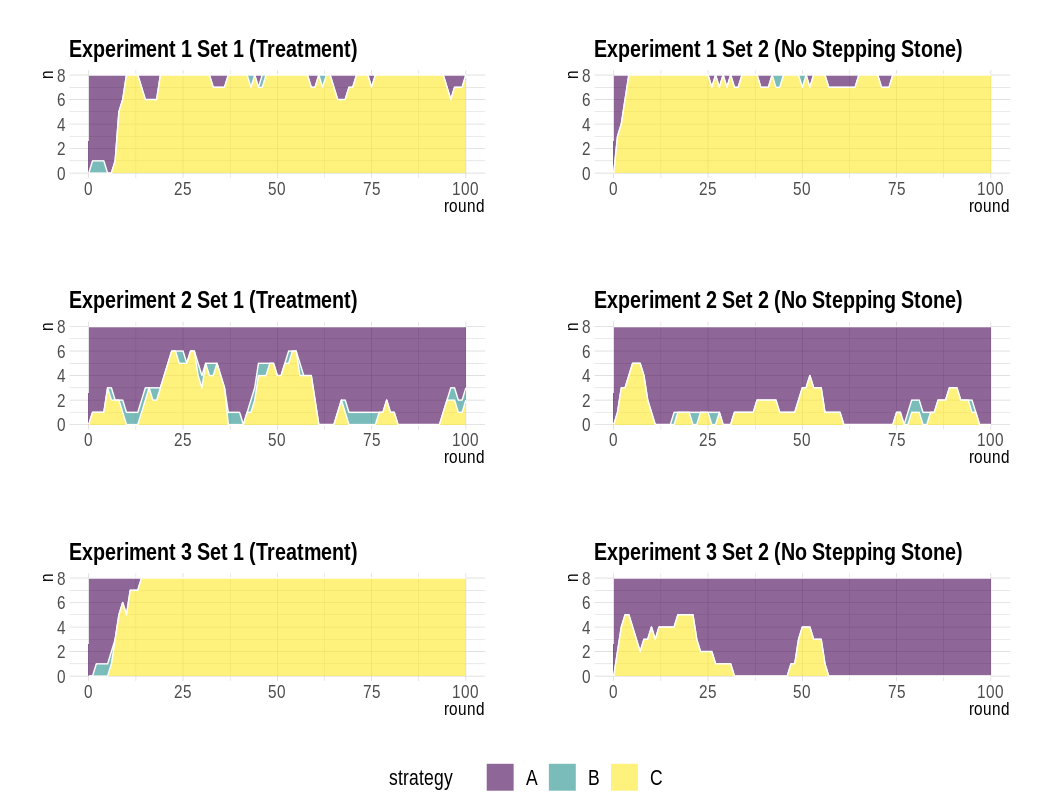
\includegraphics[width = \textwidth]{Images/AllAreaPlot1C.png}
    
\end{figure}

\begin{figure}[h]
\captionsetup{justification=centering}
  \caption{No Stepping Stone \& Incomplete Information Time Series of Group Strategy}
   \label{fig:Series1I}
    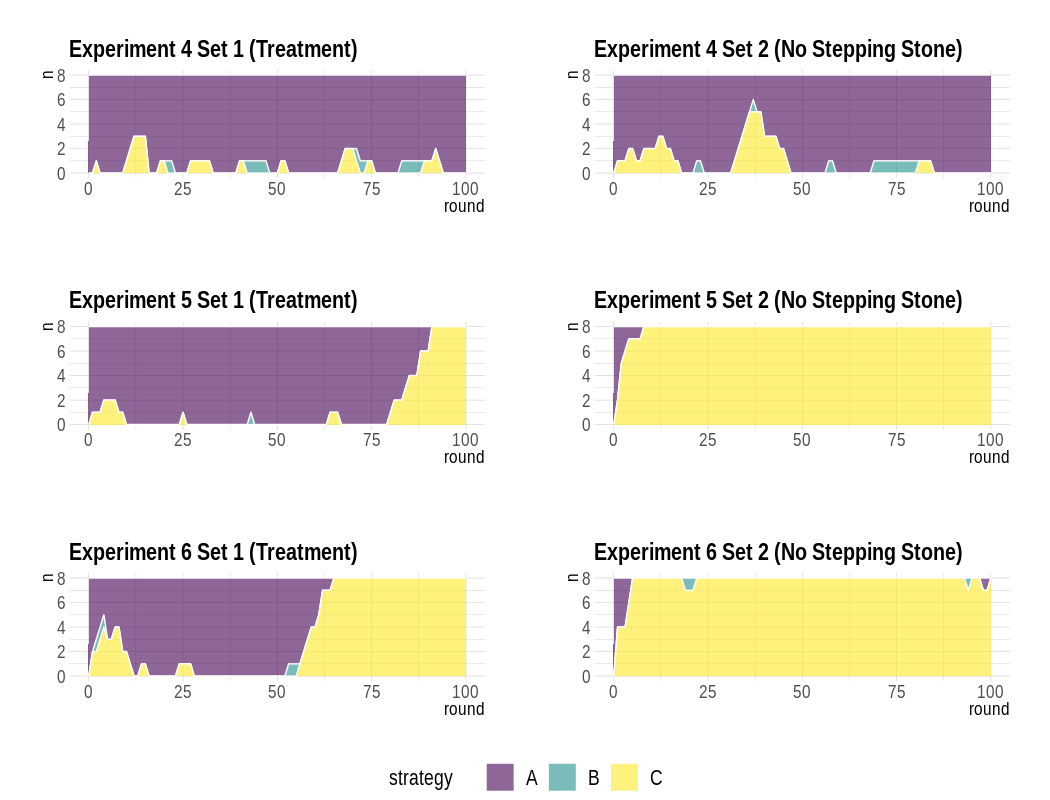
\includegraphics[width = \textwidth]{Images/AllAreaPlot1I.png}
    
\end{figure}

\begin{figure}[h]
\captionsetup{justification=centering}
  \caption{High Payoff Stepping Stone \& Complete Information Time Series of Group Strategy}
   \label{fig:Series2C}
    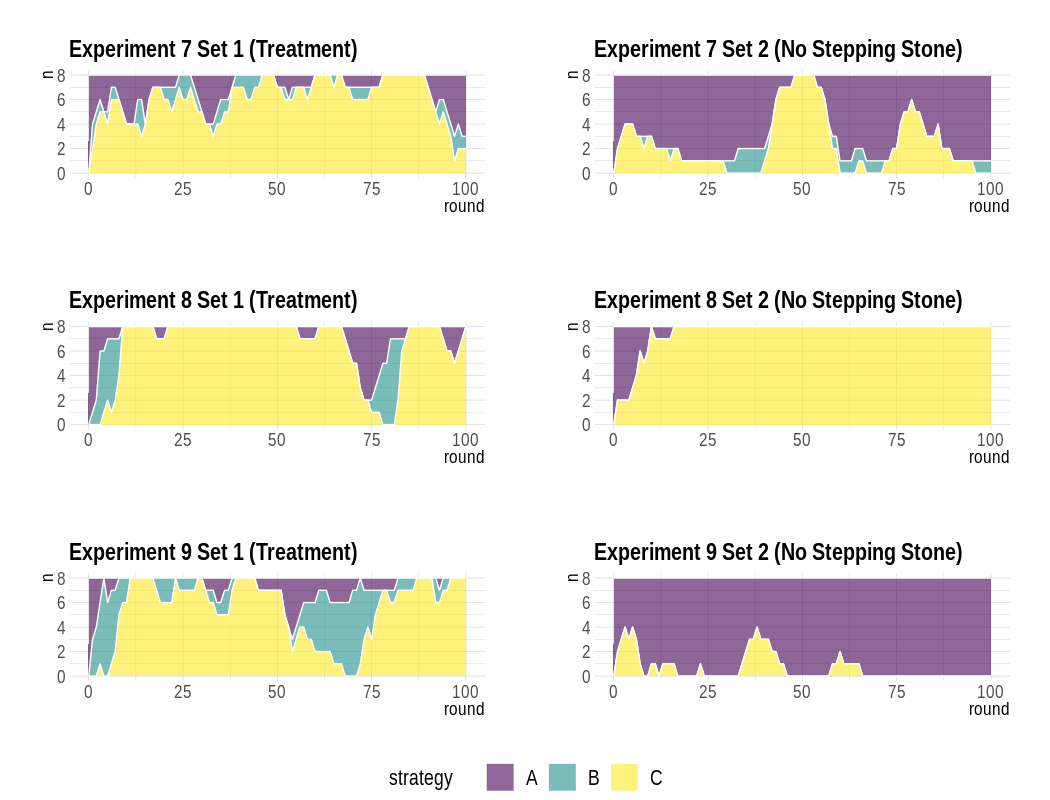
\includegraphics[width = \textwidth]{Images/AllAreaPlot2C.png}
    
\end{figure}

\begin{figure}[h]
\captionsetup{justification=centering}
  \caption{High Payoff Stepping Stone \& Incomplete Information Time Series of Group Strategy}
   \label{fig:Series2I}
    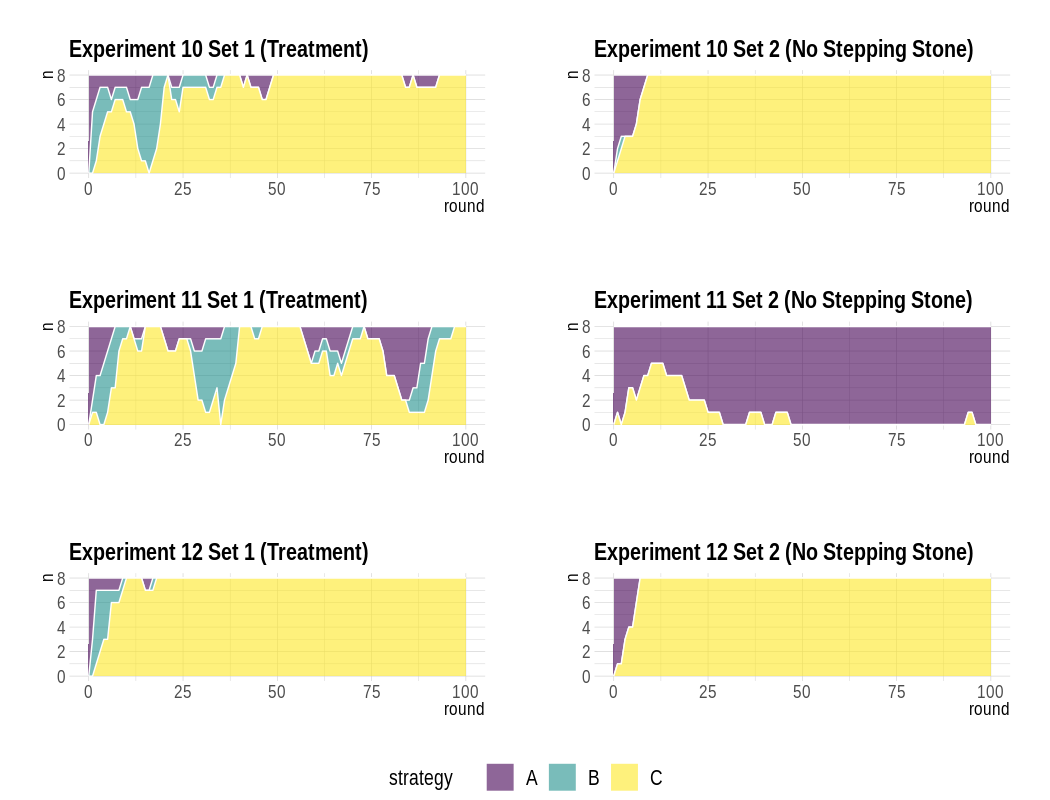
\includegraphics[width = \textwidth]{Images/AllAreaPlot2I.png}
    
\end{figure}

\begin{figure}[h]
\captionsetup{justification=centering}
  \caption{Low Payoff Stepping Stone \& Complete Information Time Series of Group Strategy}
   \label{fig:Series3C}
    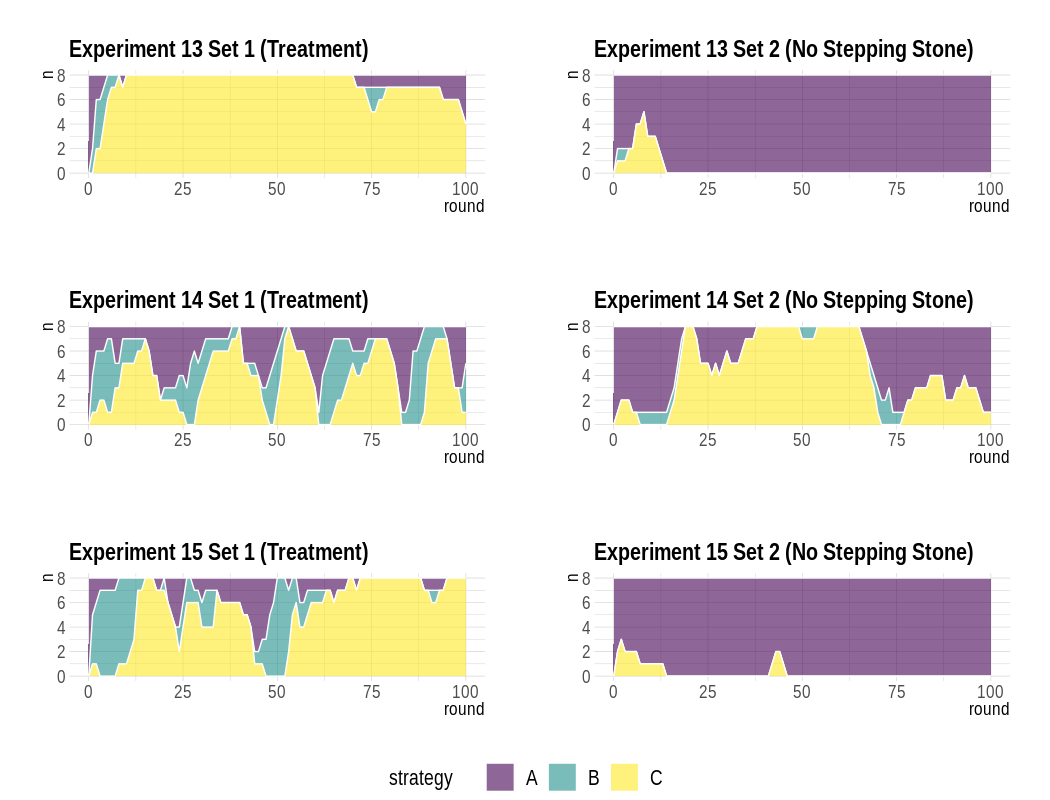
\includegraphics[width = \textwidth]{Images/AllAreaPlot3C.png}
    
\end{figure}

\begin{figure}[h]
\captionsetup{justification=centering}
  \caption{Low Payoff Stepping Stone \& Incomplete Information Time Series of Group Strategy}
   \label{fig:Series3I}
    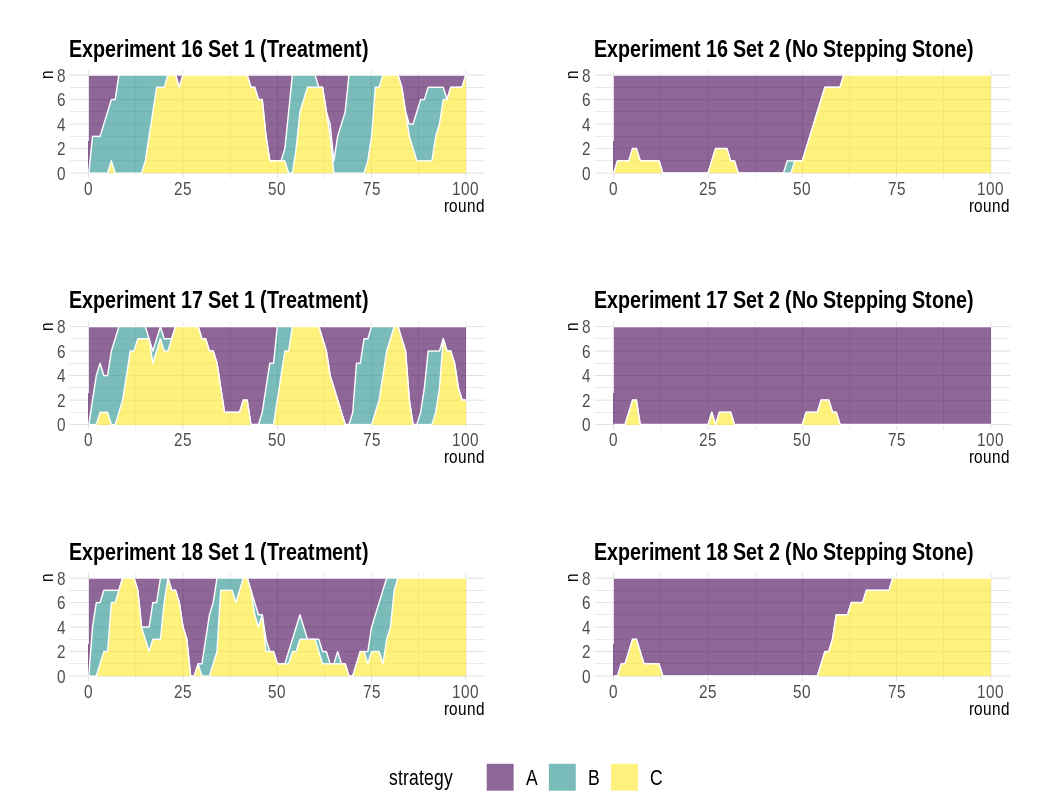
\includegraphics[width = \textwidth]{Images/AllAreaPlot3I.png}
    
\end{figure}

\begin{table}[h]
\centering
\caption{Proportion of Strategy A, B, and C Played in Each Session}
\label{tab:propstrateach}
\begin{tabular}{ c c c c c c c c c} 
\Xhline{.1em}
\multirow{2}{8em}{Game} & \multirow{2}{5em}{Information} & \multirow{2}{1em}{\#} & \multicolumn{3}{c}{Set 1: Treatment} & \multicolumn{3}{c}{Set 2: Effects}\\
& & & A & B & C & A & B & C \\
\hline
\multirow{6}{8em}{No Stepping Stone} & \multirow{3}{0em}{I} & 1 & \textcolor{red}{0.924} & 0.021 & 0.055 & \textcolor{red}{0.879} & 0.021 & 0.1 \\ 
& & 2 & \textcolor{red}{0.828} & 0.001 & 0.171 & 0.019 & 0 & \textcolor{red}{0.981}\\ 
& & 3 & \textcolor{red}{0.537} & 0.007 & 0.455 & 0.02  & 0.005 & \textcolor{red}{0.975}\\ 
%\cline{2-9}
 & \multirow{3}{0em}{C} & 1 & 0.11 & 0.009 & \textcolor{red}{0.881} & 0.039 & 0.004 & \textcolor{red}{0.958} \\  
& & 2 & \textcolor{red}{0.696} & 0.051 & 0.252 & \textcolor{red}{0.835} & 0.015 & 0.15 \\ 
& & 3 & 0.072 & 0.006 & \textcolor{red}{0.921} & \textcolor{red}{0.843} & 0 & 0.158\\ 
%\cline{1-9}
\multirow{6}{8em}{High Payoff Stepping Stone} & \multirow{3}{0em}{I} & 1 & 0.056 & 0.105 & \textcolor{red}{0.839} & 0.041 & 0.003 & \textcolor{red}{0.956}\\ 
& & 2 & 0.159 & 0.169 & \textcolor{red}{0.672} & \textcolor{red}{0.89} & 0 & 0.11\\
& & 3 & 0.018 & 0.034 & \textcolor{red}{0.949} & 0.036 & 0 & \textcolor{red}{0.964}\\ 
%\cline{2-9}
 & \multirow{3}{0em}{C} & 1 & 0.17 & 0.075 & \textcolor{red}{0.755} & \textcolor{red}{0.649} & 0.051 & 0.3\\  
& & 2 & 0.115 & 0.086 & \textcolor{red}{0.799} & 0.056 & 0 & \textcolor{red}{0.944}\\ 
& & 3 & 0.106 & 0.219 & \textcolor{red}{0.675} & \textcolor{red}{0.92} & 0 & 0.08\\ 
%\cline{1-9}
\multirow{6}{8em}{Low Payoff Stepping Stone} & \multirow{3}{0em}{I} & 1 & 0.166 & 0.295 & \textcolor{red}{0.539} & 0.494 & 0.003 & \textcolor{red}{0.504} \\ 
& & 2 & 0.325 & 0.204 & \textcolor{red}{0.471} & \textcolor{red}{0.972} & 0 & 0.028\\
& & 3 & 0.336 & 0.138 & \textcolor{red}{0.526} & \textcolor{red}{0.583} & 0 & 0.418\\ 
%\cline{2-9}
 & \multirow{3}{0em}{C} & 1 & 0.065 & 0.03 & \textcolor{red}{0.905} & \textcolor{red}{0.956} & 0.004 & 0.04\\  
& & 2 & 0.298 & 0.248 & \textcolor{red}{0.455} & 0.415 & 0.038 & \textcolor{red}{0.548}\\ 
& & 3 & 0.135 & 0.205 & \textcolor{red}{0.66} & \textcolor{red}{0.968} & 0 & 0.032\\ 
\Xhline{.1em}
\end{tabular}
\end{table}%


\begin{table}[h]
\centering
\caption{Mean Proportion of Strategy A, B, and C Played in Each Treatment}
\label{tab:propstratall}
\begin{tabular}{ c c c c c c c c} 
\Xhline{.1em}
\multirow{2}{8em}{Game} & \multirow{2}{5em}{Information} & \multicolumn{3}{c}{Set 1: Treatment} & \multicolumn{3}{c}{Set 2: Effects}\\
& & A & B & C & A & B & C \\
\hline
\multirow{2}{8em}{No Stepping Stone} & I &  \textcolor{red}{0.763} & 0.010 & 0.227 & 0.306 & 0.009 & \textcolor{red}{0.685}\\ 
 & C & 0.293 & 0.22 & \textcolor{red}{0.685} & \textcolor{red}{0.572} & 0.006 & 0.422 \\  
%\cline{1-8}
\multirow{2}{8em}{High Payoff Stepping Stone} & I & 0.078 & 0.103 & \textcolor{red}{0.82} & 0.322 & 0.001 & \textcolor{red}{0.677}\\ 
 & C & 0.13 & 0.127 & \textcolor{red}{0.743} & \textcolor{red}{0.542} & 0.017 & 0.441\\  
%\cline{1-8}
\multirow{2}{8em}{Low Payoff Stepping Stone} & I & 0.276 & 0.212 & \textcolor{red}{0.512} & \textcolor{red}{0.683} & 0.001 & 0.316\\ 
 & C & 0.166 & 0.161 & \textcolor{red}{0.673} & \textcolor{red}{0.78} & 0.014 & 0.207\\  
\Xhline{.1em}
\end{tabular}
\end{table}%

\begin{table}[h]
\footnotesize
\centering
\caption{Choices in each Session by MBR}
\label{tab:choiceexperiment}
\begin{tabular}{ c c c c c c c c c c c c} 
\Xhline{.1em}
\multirow{2}{8em}{Game} & \multirow{2}{5em}{Information} & \multirow{2}{1em}{\#} & \multirow{2}{2em}{mBR} & \multicolumn{4}{c}{Set1: Treatment} & \multicolumn{4}{c}{Set 2: Effects}\\
& & & & n & A & B & C & n & A & B & C \\
\hline
\multirow{12}{8em}{No Stepping Stone} & \multirow{6}{0em}{I} & \multirow{2}{0em}{1} & A & 800 & .93 & .02 & .05 & 798 & .9 & .01 & .09 \\ 
& & & C & 0 & - & - & - & 2 & .5 & 0 & .5 \\
& & \multirow{2}{0em}{2} & A & 722 & .89 & 0 & .11 & 30 & .13 & 0 & .87 \\ 
& & & C & 78 & .03 & 0 & 0 & 770 & 0 & 0 & 1 \\
& & \multirow{2}{0em}{3} & A & 496 & .86 & .01 & .13 & 38 & .18 & 0 & .82 \\ 
& & & C & 304 & 0 & 0 & 1 & 762 & 0 & .01 & .99 \\
%\cline{2-12}
 & \multirow{6}{0em}{C} & \multirow{2}{0em}{1} & A & 126 & .4 & .01 & .59 & 30 & .23 & 0 & .77 \\ 
& & & C & 674 & .05 & 0 & .95 & 770 & .02 & .01 & .97 \\ 
& & \multirow{2}{0em}{2} & A & 782 & .7 & .05 & .25 & 800 & .84 & .02 & .14 \\ 
& & & C & 18 & .67 & 0 & .33 & 0 & - & - & - \\
& & \multirow{2}{0em}{3} & A & 593 & .59 & .03 & .37 & 800 & .82 & 0 & .18 \\ 
& & & C & 714 & 0 & 0 & 1 & 0 & - & - & - \\
%\cline{1-9}
\multirow{18}{8em}{High Payoff Stepping Stone} & \multirow{9}{0em}{I} & \multirow{3}{0em}{1} & A & 34 & .18 & .35 & .47 & 62 & .4 & .02 & .58 \\ 
& & & B & 56 & .02 & .66 & .32 & - & - & - & - \\ 
& & & C & 710 & .04 & .03 & .93 & 738 & 0 & 0 & 1 \\
& & \multirow{3}{0em}{2} & A & 152 & .38 & .11 & .51 & 800 & .91 & 0 & .09 \\ 
& & & B & 102 & .08 & .67 & .25 & - & - & - & - \\ 
& & & C & 546 & .08 & .07 & .85 & 0 & - & - & - \\ 
& & \multirow{3}{0em}{3} & A & 8 & .25 & .62 & .12 & 54 & .43 & 0 & .57 \\ 
& & & B & 18 & .11 & .56 & .33 & - & - & - & - \\ 
& & & C & 774 & .01 & .01 & .98 & 746 & 0 & 0 & 1 \\ 
& \multirow{9}{0em}{C} & \multirow{3}{0em}{1} & A & 210 & .29 & .16 & .55 & 698 & .73 & .06 & .21 \\ 
& & & B & 21 & .29 & .19 & .52 & - & - & - & - \\ 
& & & C & 569 & .11 & .07 & .82 & 102 & .11 & 0 & .89 \\
& & \multirow{3}{0em}{2} & A & 100 & .52 & .16 & .32 & 76 & .42 & 0 & .58 \\ 
& & & B & 82 & .07 & .68 & .24 & - & - & - & - \\ 
& & & C & 674 & .04 & 0 & .96 & 724 & 0 & 0 & 1 \\ 
& & \multirow{3}{0em}{3} & A & 62 & .5 & .19 & .31 & 800 & .92 & 0 & .07 \\ 
& & & B & 138 & .14 & .69 & .17 & - & - & - & - \\ 
& & & C & 600 & .06 & .1 & .84 & 0 & - & - & - \\
%\cline{1-9}
\multirow{18}{8em}{Low Payoff Stepping Stone} & \multirow{9}{0em}{I} & \multirow{3}{0em}{1} & A & 116 & .63 & .28 & .09 & 446 & .87 & 0 & .13 \\ 
& & & B & 256 & .04 & .79 & .17 & - & - & - & - \\ 
& & & C & 428 & .1 & .02 & .88 & 354 & .01 & 0 & .99 \\
& & \multirow{3}{0em}{2} & A & 268 & .76 & .13 & .11 & 800 & .98 & 0 & .02 \\ 
& & & B & 175 & .06 & .74 & .19 & - & - & - & - \\ 
& & & C & 357 & .1 & .02 & .87 & 0 & - & - & - \\ 
& & \multirow{3}{0em}{3} & A & 316 & .69 & .12 & .18 & 528 & .84 & 0 & .16 \\ 
& & & B & 103 & .08 & .54 & .38 & - & - & - & - \\ 
& & & C & 381 & .06 & .04 & .9 & 272 & .03 & 0 & .97 \\ 
& \multirow{9}{0em}{C} & \multirow{3}{0em}{1} & A & 48 & .21 & .1 & .69 & 800 & .95 & 0 & .05 \\ 
& & & B & 18 & .17 & .56 & .28 & - & - & - & - \\ 
& & & C & 734 & .05 & .01 & .93 & 0 & - & - & - \\
& & \multirow{3}{0em}{2} & A & 256 & .54 & .21 & .26 & 498 & .64 & .04 & .32 \\ 
& & & B & 209 & .15 & .62 & .23 & - & - & - & - \\ 
& & & C & 335 & .21 & .07 & .72 & 302 & .04 & .02 & .94 \\
& & \multirow{3}{0em}{3} & A & 124 & .38 & .16 & .46 & 800 & .97 & 0 & .03 \\ 
& & & B & 144 & .1 & 0 & .18 & - & - & - & - \\ 
& & & C & 532 & .09 & .04 & .87 & 0 & - & - & - \\ 
\Xhline{.1em}
\end{tabular}
\end{table}%

\begin{table}[h] \centering 
  \caption{Grouped Choices by Treatment}
  \label{tab:groupedchoicetreat} 
\begin{tabular}{@{\extracolsep{5pt}} cccccccc} 
\Xhline{.1em}
Game & Information & mBR & n & A & B & C \\ 
\hline \\[-1.8ex] 
\multirow{4}{8em}{No Stepping Stone}& C & A & 994 & 0.65 & 0.04 & 0.3 \\ 
 & C & C & 1406 & 0.03 & 0 & 0.96 \\ 
 & I & A & 2018 & 0.9 & 0.01 & 0.09 \\ 
& I & C & 382 & 0.01 & 0 & 0.99 \\ 
\multirow{6}{8em}{High Payoff Stepping Stone} & C & A & 372 & 0.39 & 0.16 & 0.45 \\ 
& C & B & 241 & 0.13 & 0.64 & 0.22 \\ 
& C & C & 1787 & 0.07 & 0.06 & 0.87 \\ 
& I & A & 194 & 0.34 & 0.18 & 0.48 \\ 
 & I & B & 176 & 0.06 & 0.65 & 0.28 \\ 
 & I & C & 2030 & 0.04 & 0.03 & 0.93 \\ 
\multirow{6}{8em}{Low Payoff Stepping Stone} & C & A & 428 & 0.45 & 0.18 & 0.36 \\ 
 & C & B & 371 & 0.13 & 0.65 & 0.22 \\ 
& C & C & 1601 & 0.1 & 0.03 & 0.87 \\ 
& I & A & 700 & 0.71 & 0.15 & 0.14 \\ 
 & I & B & 534 & 0.05 & 0.73 & 0.22 \\ 
 & I & C & 1166 & 0.09 & 0.03 & 0.88 \\ 
\hline \\[-1.8ex] 
\end{tabular} 
\end{table} 

\begin{table}[!htbp]
\caption{Generalized Logistic Mixed Model: Is $C$ Played More in Game 2 and 3 than Game 1?}
\label{regression:logit1} 
\centering
\begin{tabular}{lllll}
\hline
\textbf{Fixed Effects} & \textbf{Estimate} & \textbf{Std. Error} & \textbf{z value} & \textbf{Pr($>|z|$)} \\
\hline
(Intercept) & -0.3045 & 0.2230 & -1.366 & 0.17202 \\
Game 2 & 1.8157 & 0.3147 & 5.770 & $7.94 \times 10^{-9}$ \\
Game 3 & 0.8588 & 0.3130 & 2.744 & 0.00608 \\
\hline
\multicolumn{5}{l}{\textbf{Model Information}} \\
\hline
AIC: 14738.0 \\
BIC: 14775.8 \\
Log Likelihood: -7364.0 \\
Deviance: 14728.0 \\
Residual degrees of freedom: 14395 \\
\hline
\end{tabular}
\end{table}

\begin{table}[htbp]
\centering
\caption{Hypothesis 3 Test: Generalized Logistic Mixed Model Results}
Data filtered to only include observations where mBR = $A$
\label{tab:regression4}
\begin{tabular}{lllll}
\hline
\textbf{Fixed Effects} & \textbf{Estimate} & \textbf{Std. Error} & \textbf{z value} & \textbf{Pr($>|z|$)} \\
\hline
(Intercept) & -1.7481 & 0.2022 & -8.645 & $<2 \times 10^{-16}$ \\
Game 3 & -0.1030 & 0.2645 & -0.389 & 0.697 \\
\hline
\multicolumn{5}{l}{\textbf{Model Information}} \\
\hline
AIC: 1448.1 \\
BIC: 1464.4 \\
Log Likelihood: -721.1 \\
Deviance: 1442.1 \\
Residual degrees of freedom: 1691 \\
\hline
\end{tabular}
\end{table}

\begin{table}[h]
\centering
\caption{Hypotheses 4, 5 and 7 Test: Generalized Logistic Mixed Model}
$mBR$ is the Dependant Variable
\label{tab:glm46}
\begin{tabular}{lllll}
\hline
\textbf{Fixed Effects} & \textbf{Estimate} & \textbf{Std. Error} & \textbf{z value} & \textbf{Pr($>|z|$)} \\
\hline
(Intercept) & -2.359739 & 0.244356 & -9.657 & $< 2 \times 10^{-16}$ \\
mBR = B & 1.200690 & 0.127741 & 9.399 & $< 2 \times 10^{-16}$ \\
mBR = C & 2.239175 & 0.097942 & 22.862 & $< 2 \times 10^{-16}$ \\
Incomplete Info & 0.741663 & 0.210947 & 3.516 & 0.000438 \\
Game 2 & 0.097101 & 0.247757 & 0.392 & 0.695116 \\
Game 3 & 0.168979 & 0.245713 & 0.688 & 0.491637 \\
lag(stochastic rejection) & 0.260193 & 0.053658 & 4.849 & $1.24 \times 10^{-6}$ \\
$\Delta\Pi_{mBR}$ & 0.110395 & 0.004179 & 26.416 & $< 2 \times 10^{-16}$ \\
log(round) & 0.290226 & 0.029797 & 9.740 & $< 2 \times 10^{-16}$ \\
mBR = B:Incomplete Info & -0.541791 & 0.173655 & -3.120 & 0.001809 \\
mBR = C:Incomplete Info & -0.582463 & 0.141303 & -4.122 & $3.75 \times 10^{-5}$ \\
\hline
\multicolumn{5}{l}{\textbf{Model Information}} \\
\hline
AIC: 9536.0 \\
BIC: 9634.3 \\
Log Likelihood: -4755.0 \\
Deviance: 9510.0 \\
Residual degrees of freedom: 14243 \\
\hline
\end{tabular}
\end{table}

\begin{figure}[h]
\captionsetup{justification=centering}
  \caption{Experiment Instructions (Complete Information)}
   \label{fig:Instructions}
    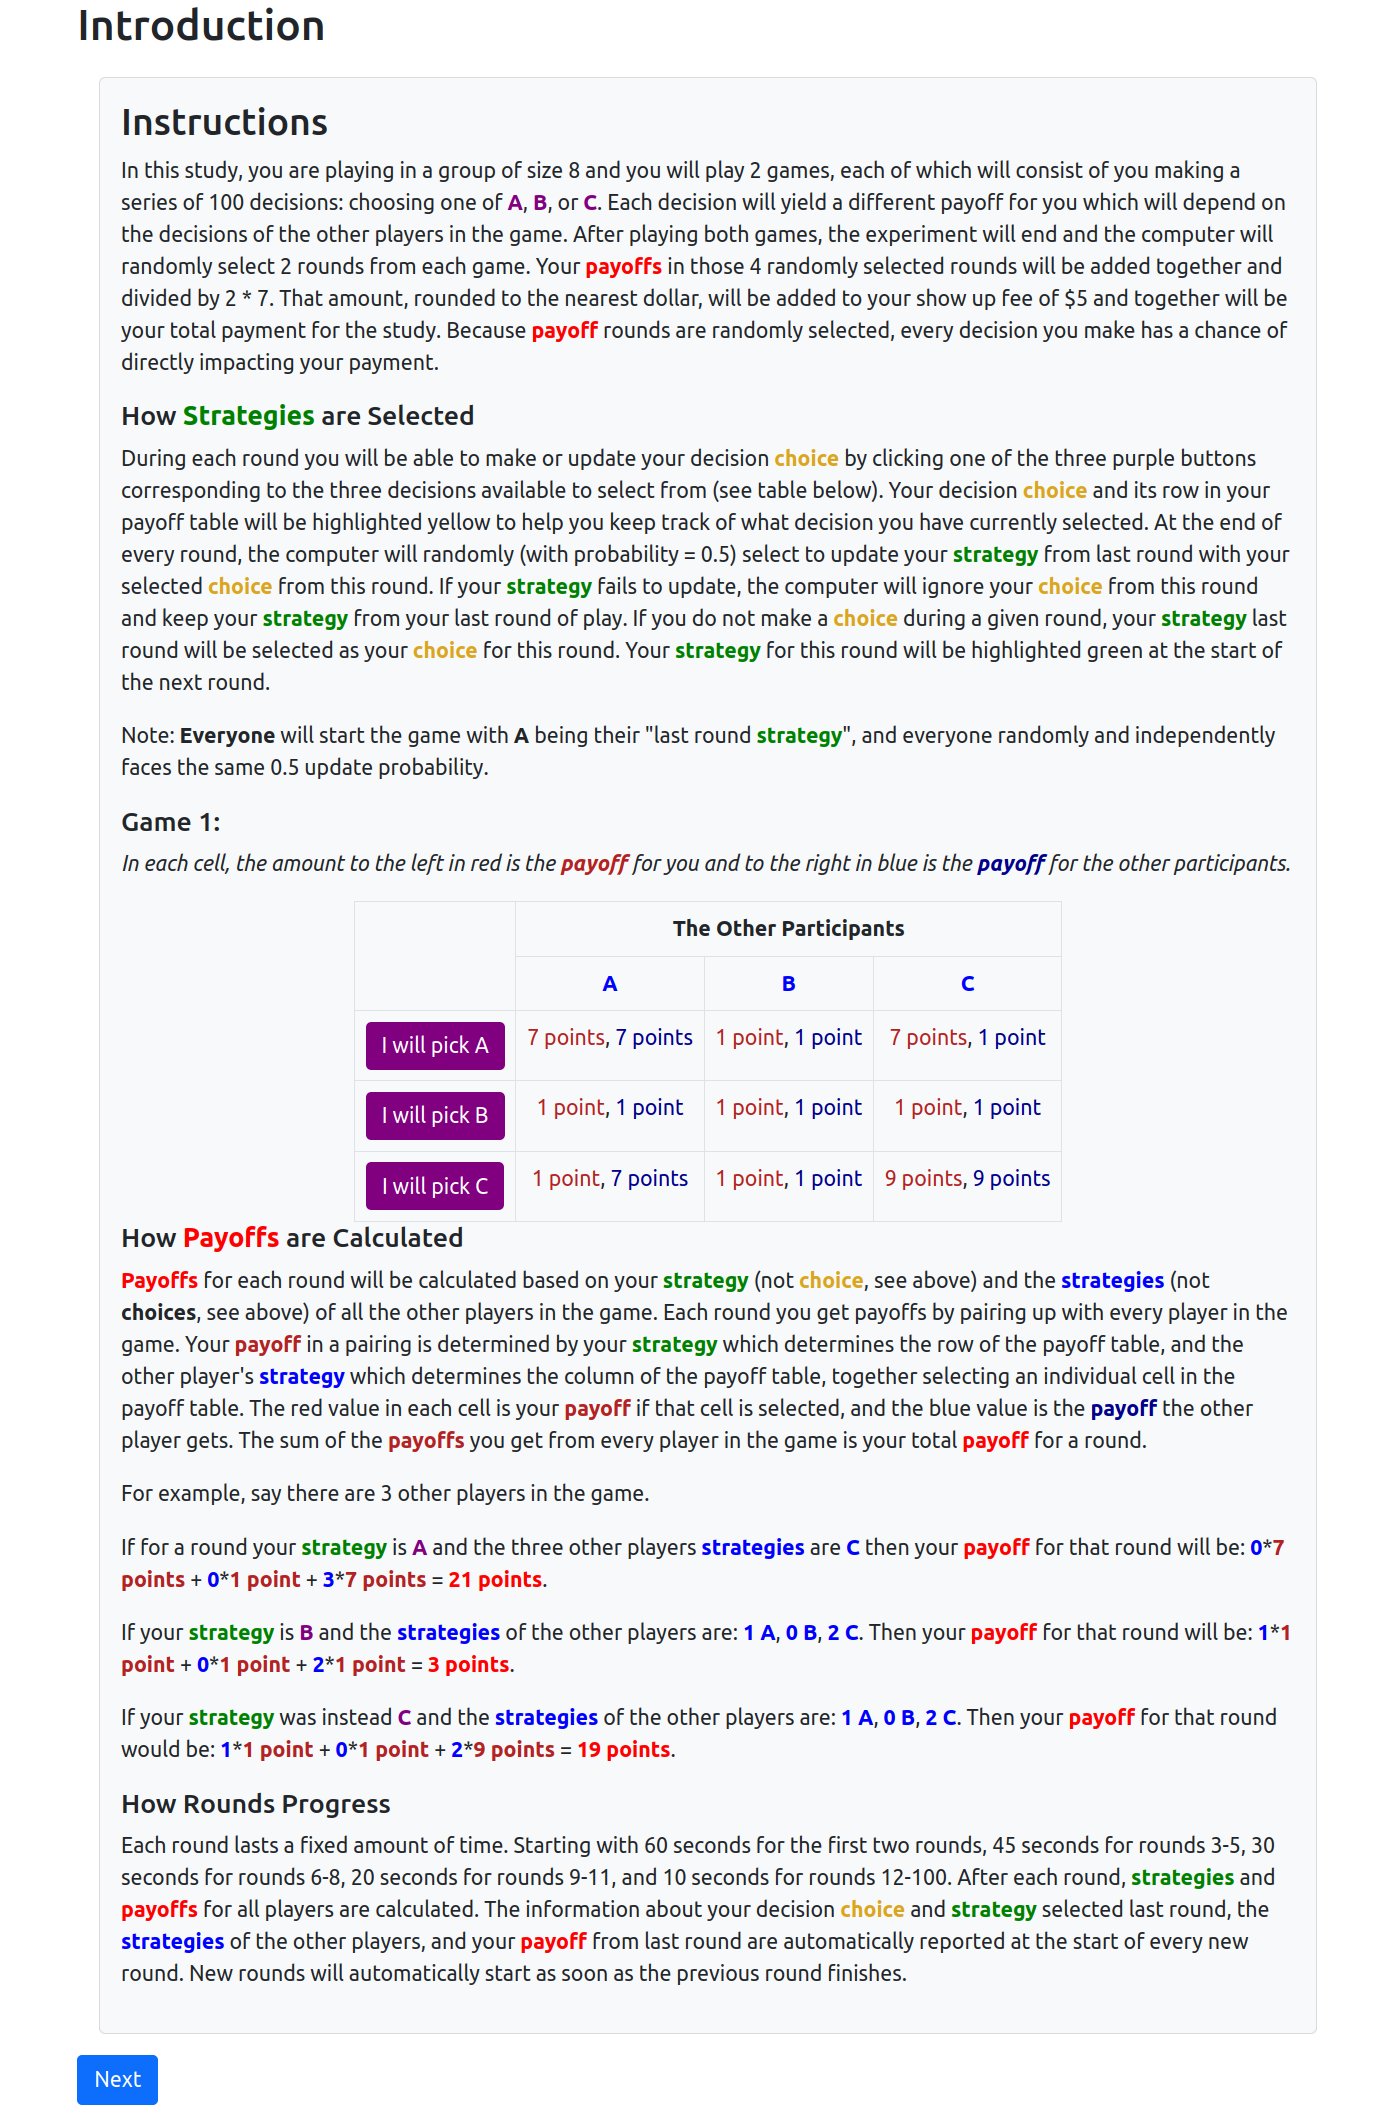
\includegraphics[width = .9\textwidth]{Images/Instructions.png}
\end{figure}

\begin{figure}[h]
\captionsetup{justification=centering}
  \caption{Quiz Question 1}
   \label{fig:QuizQ1}
    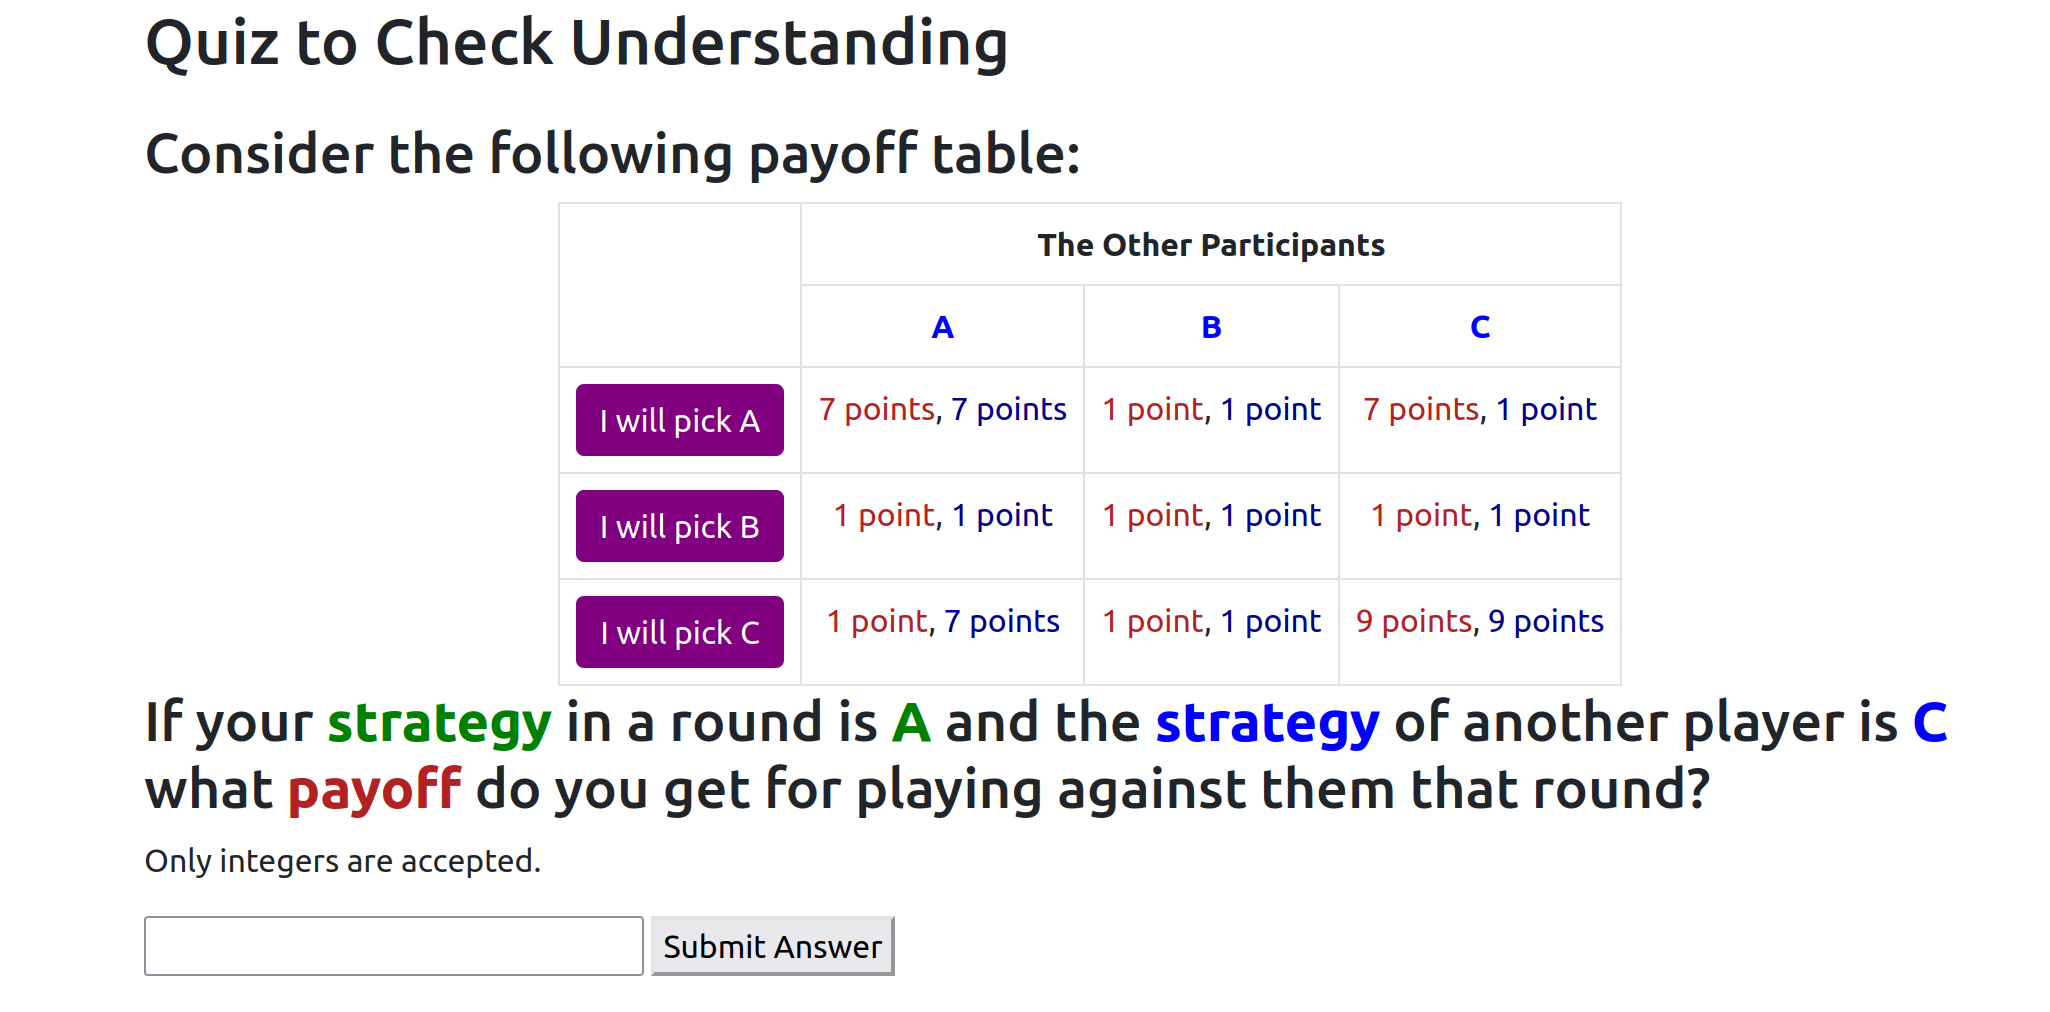
\includegraphics[width = \textwidth]{Images/Q1.png}
\end{figure}

\begin{figure}[h]
\captionsetup{justification=centering}
  \caption{Quiz Question 2 (Complete Information Only)}
   \label{fig:QuizQ2}
    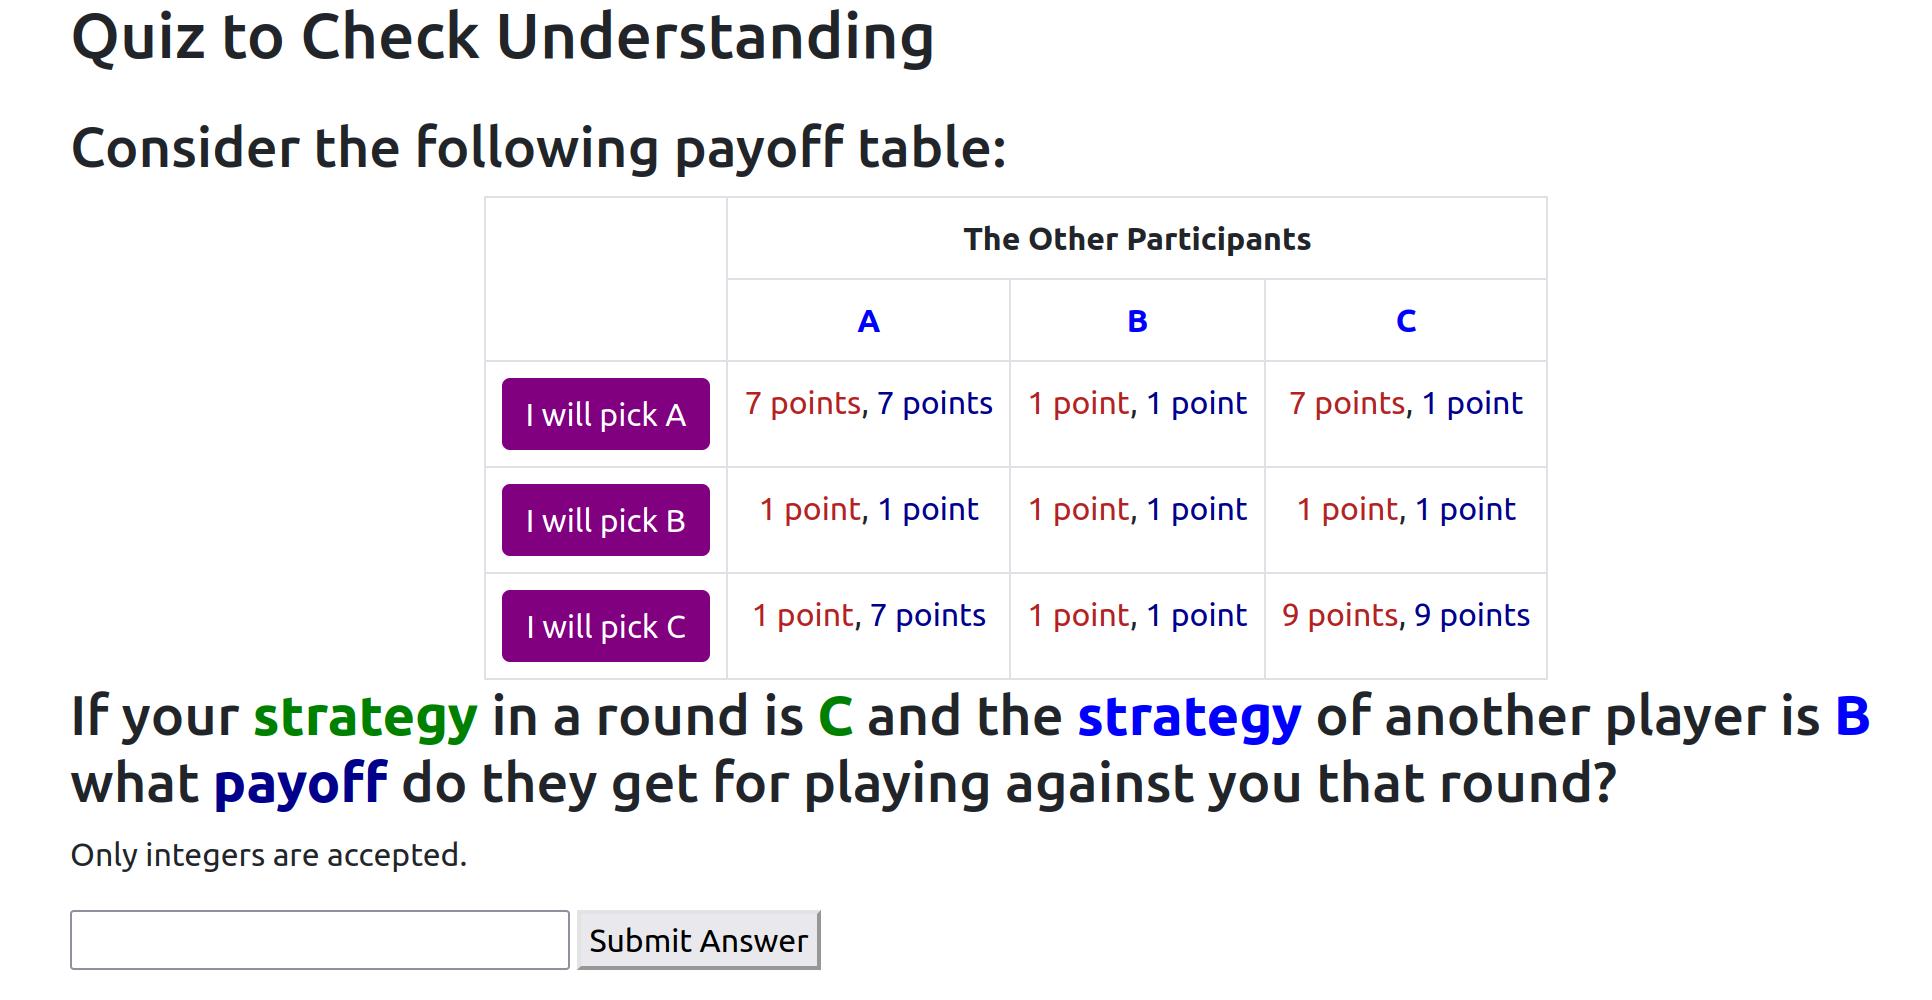
\includegraphics[width = \textwidth]{Images/Q2.png}  
\end{figure}

\begin{figure}[h]
\captionsetup{justification=centering}
  \caption{Quiz Question 3}
   \label{fig:QuizQ3}
    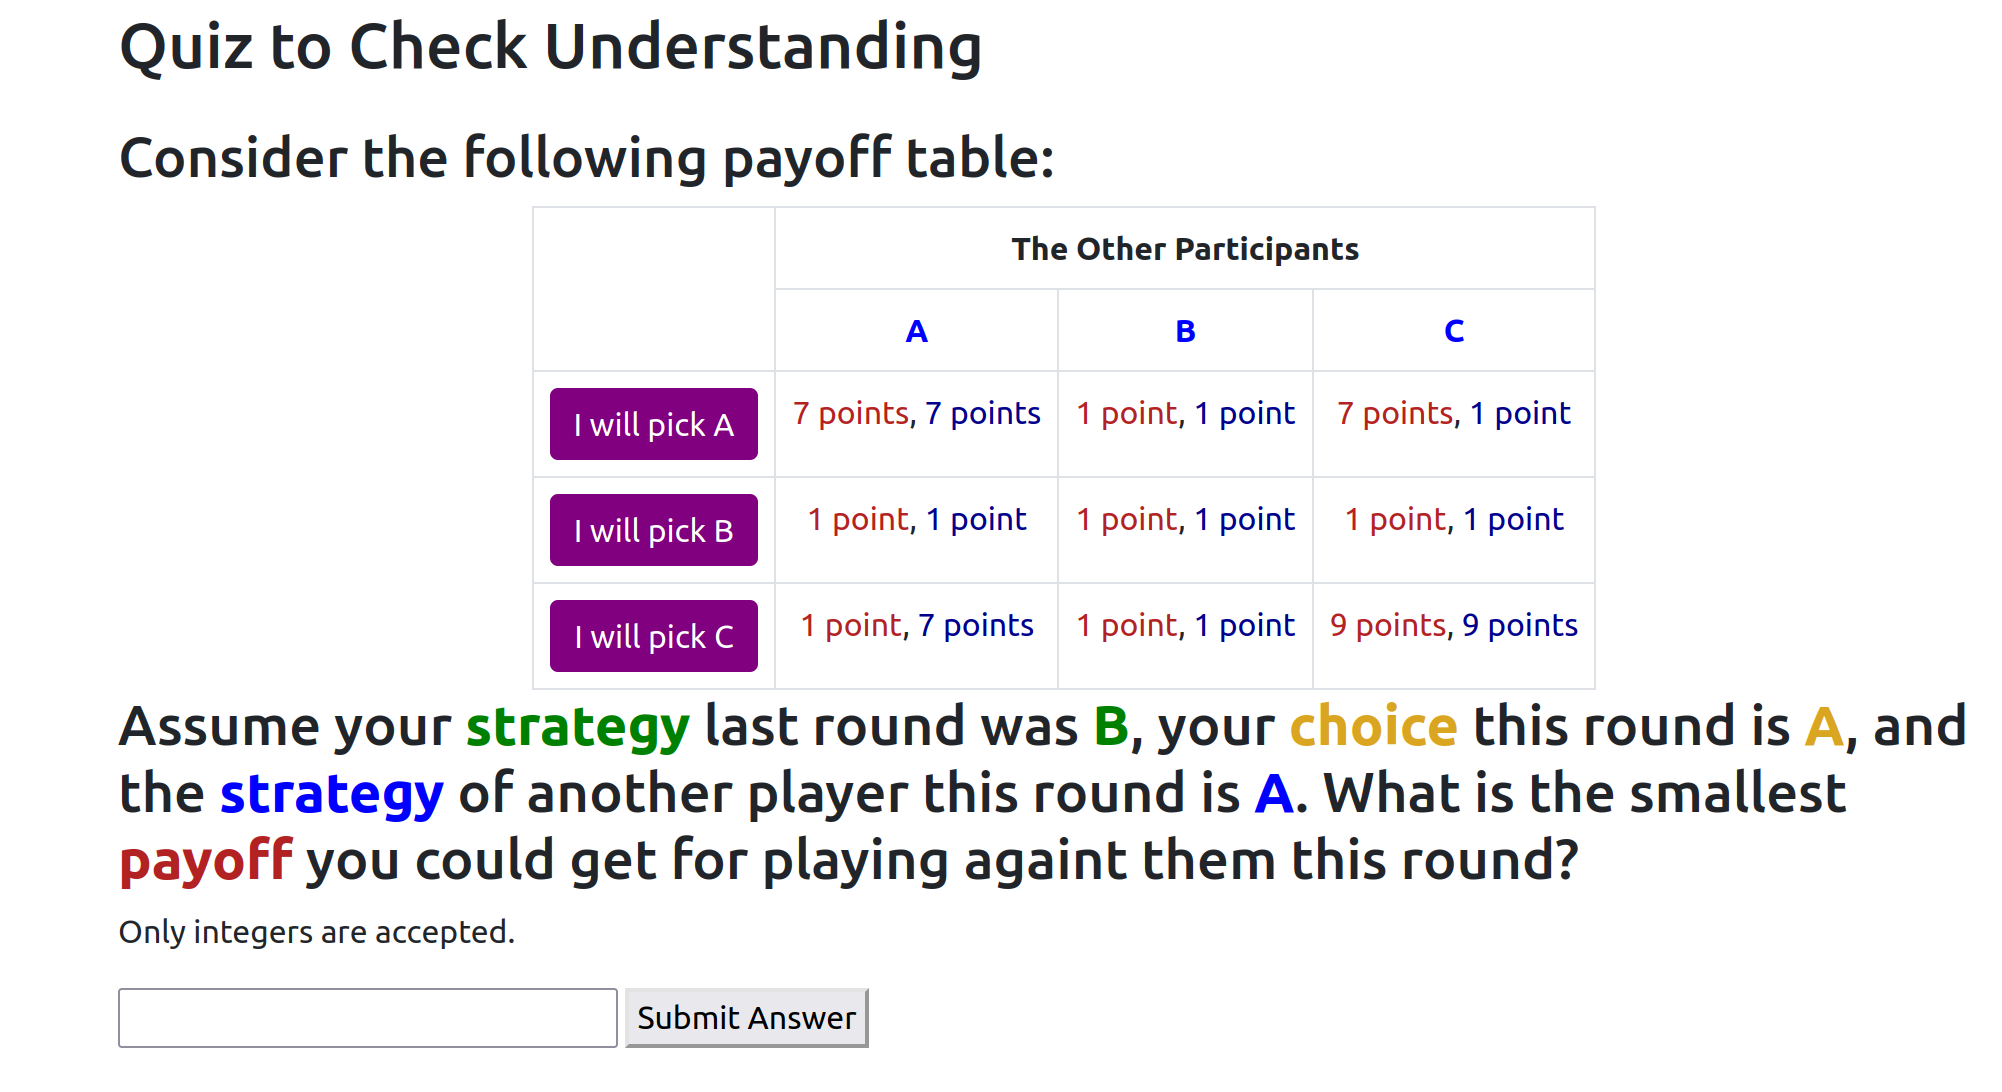
\includegraphics[width = \textwidth]{Images/Q3.png}
\end{figure}

\begin{figure}[h]
\captionsetup{justification=centering}
  \caption{Quiz Question 4}
   \label{fig:QuizQ4}
    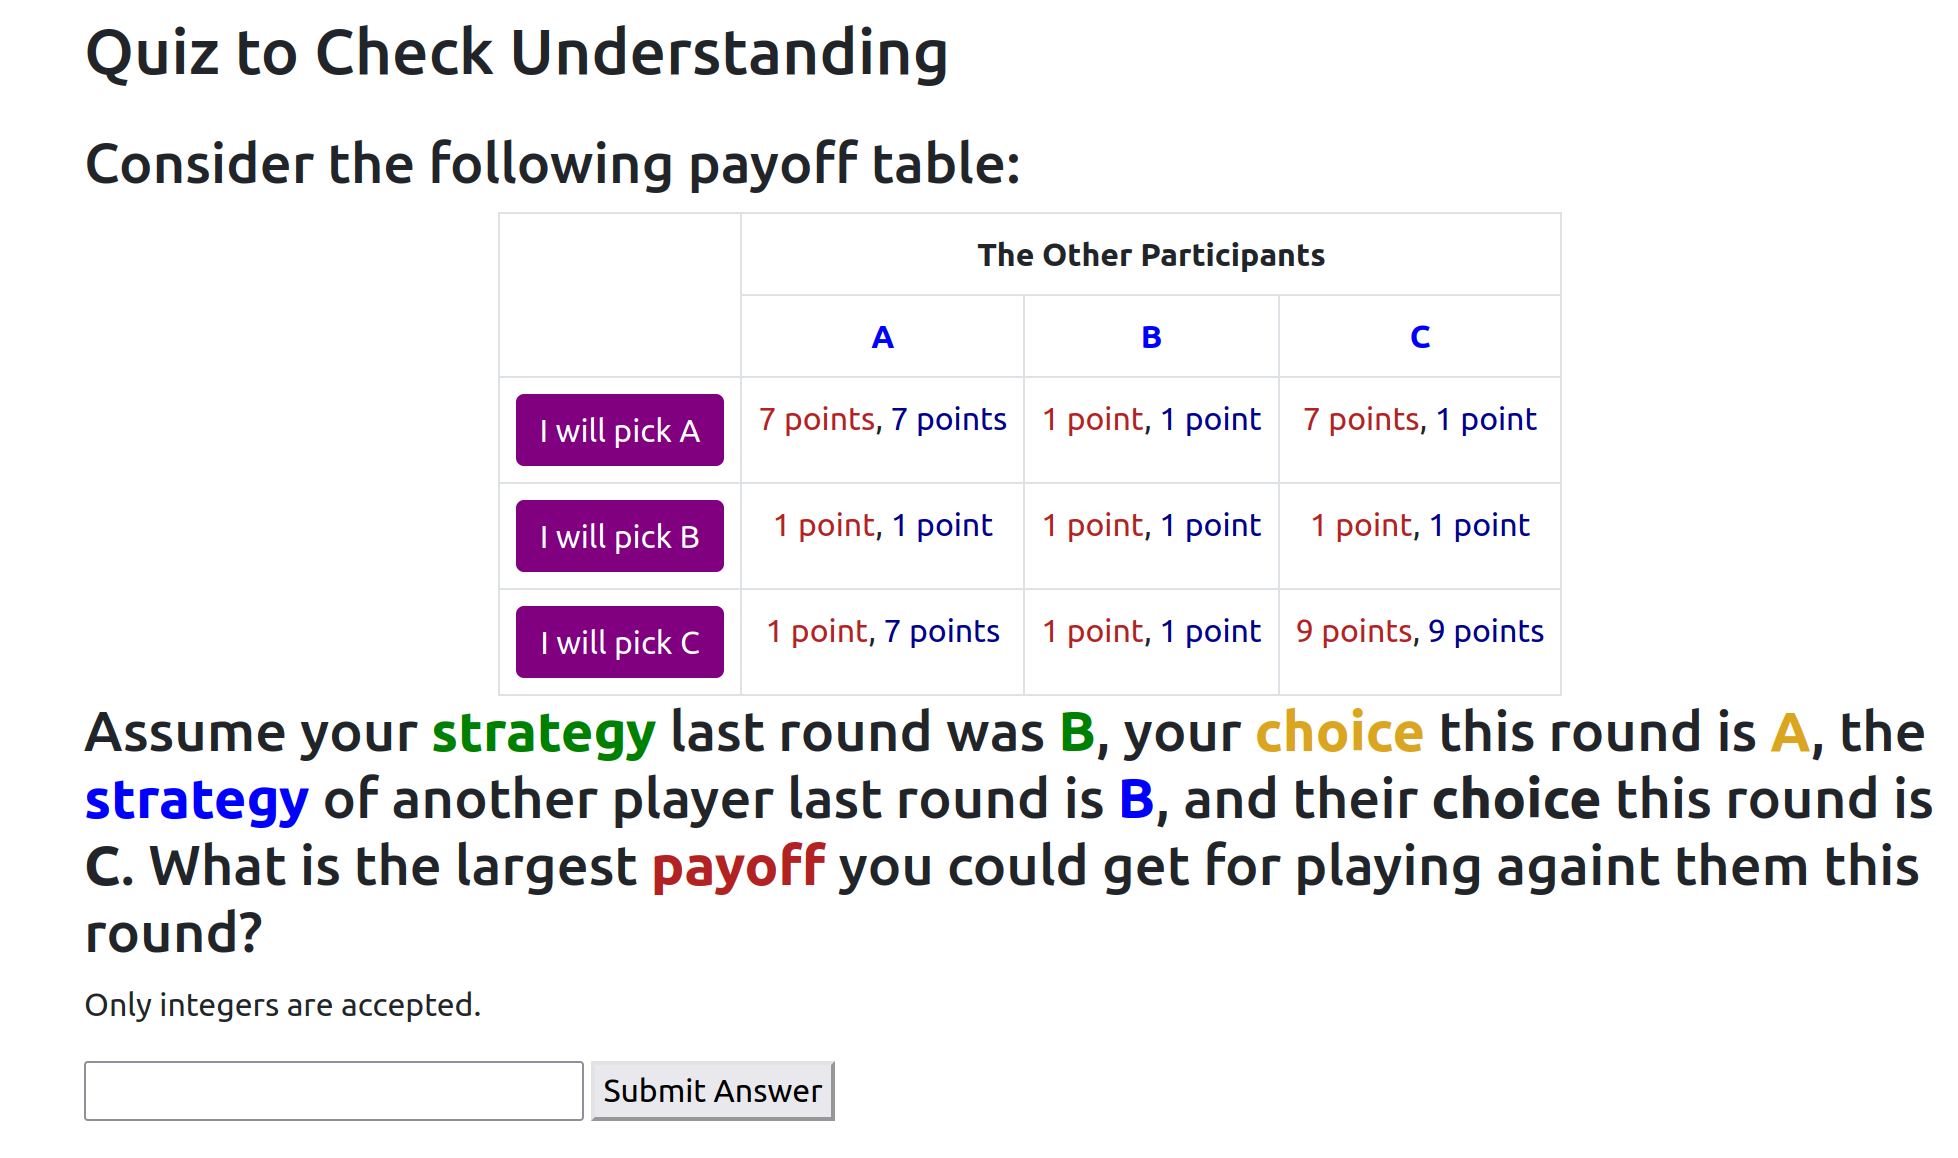
\includegraphics[width = \textwidth]{Images/Q4.png}
\end{figure}

\begin{figure}[h]
\captionsetup{justification=centering}
  \caption{Quiz Question 5}
   \label{fig:QuizQ5}
    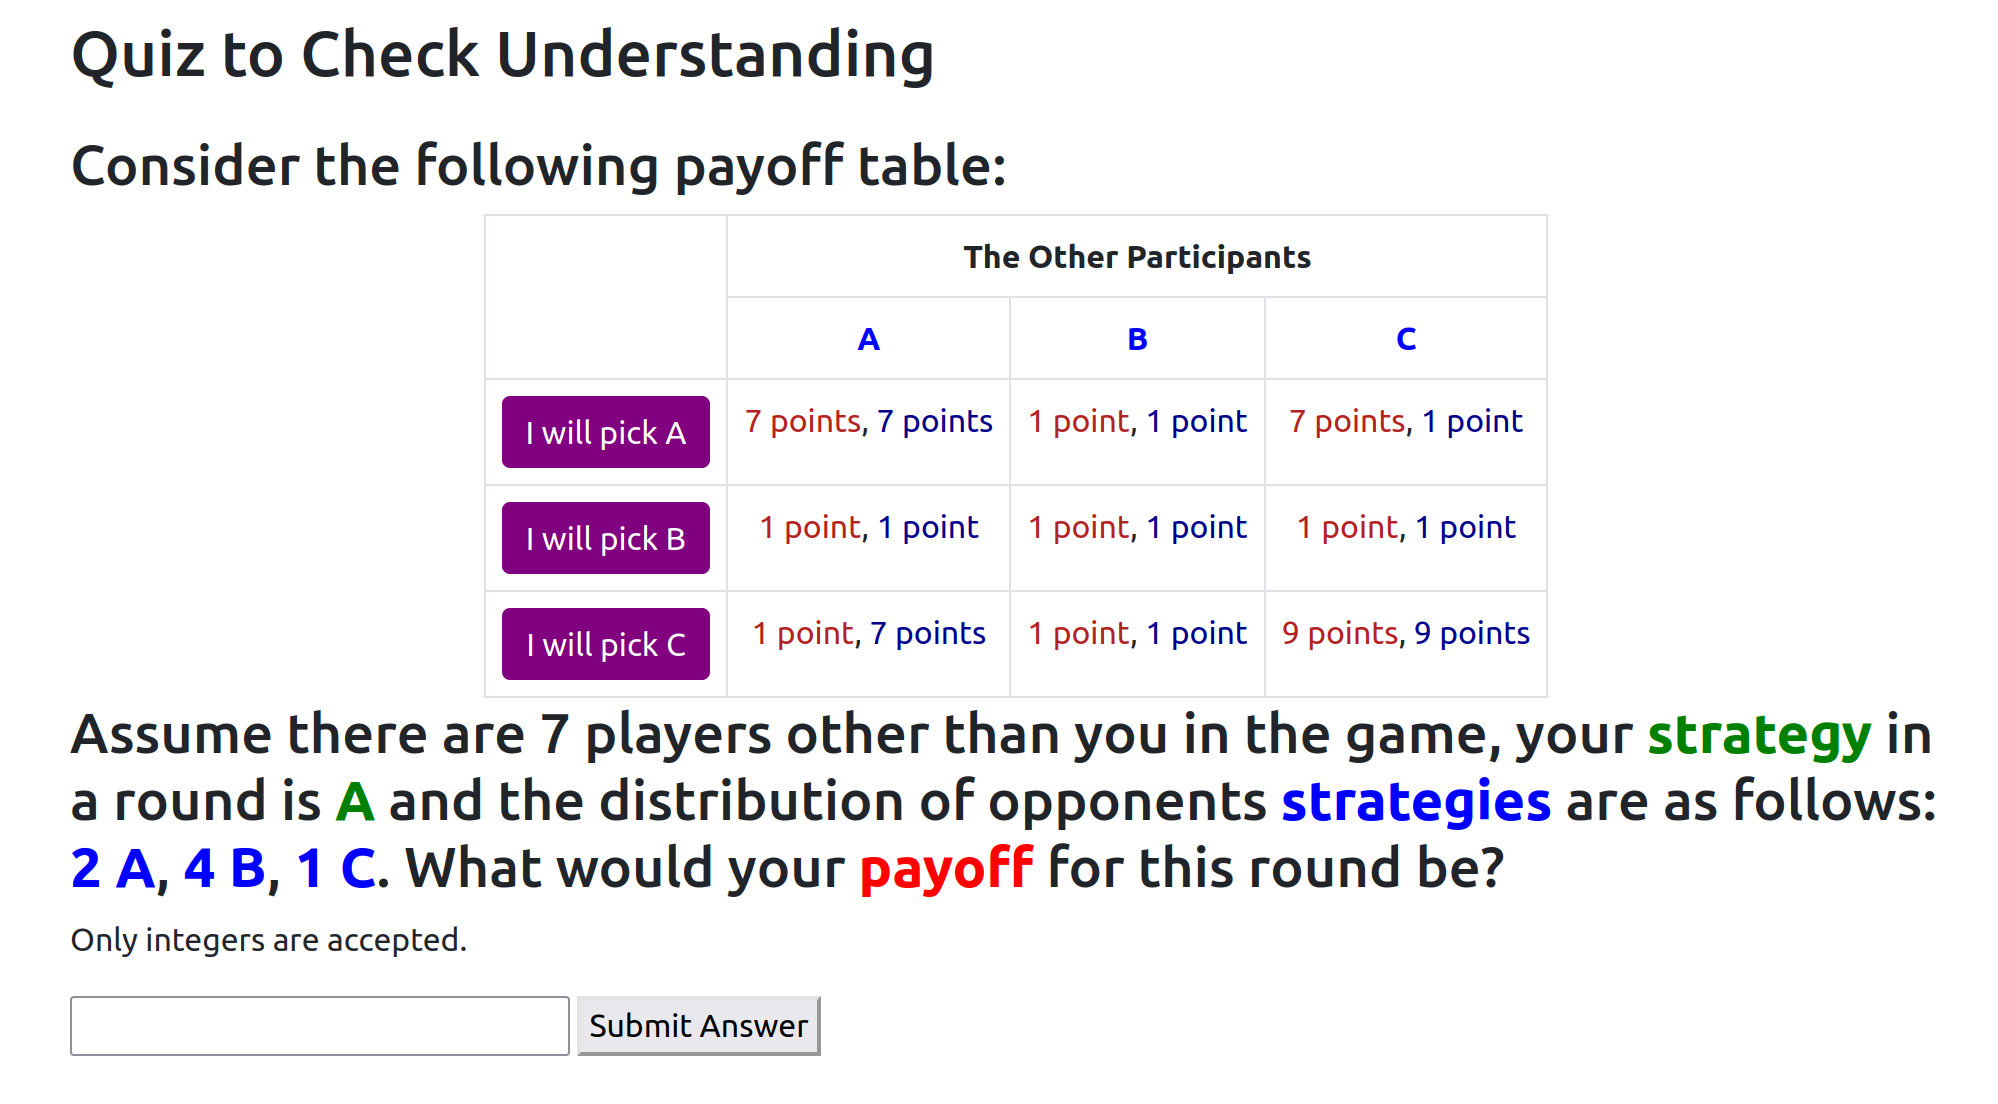
\includegraphics[width = \textwidth]{Images/Q5.png}    
\end{figure}

\begin{figure}[h]
\captionsetup{justification=centering}
  \caption{Experiment UI 1}
   \label{fig:UI1}
    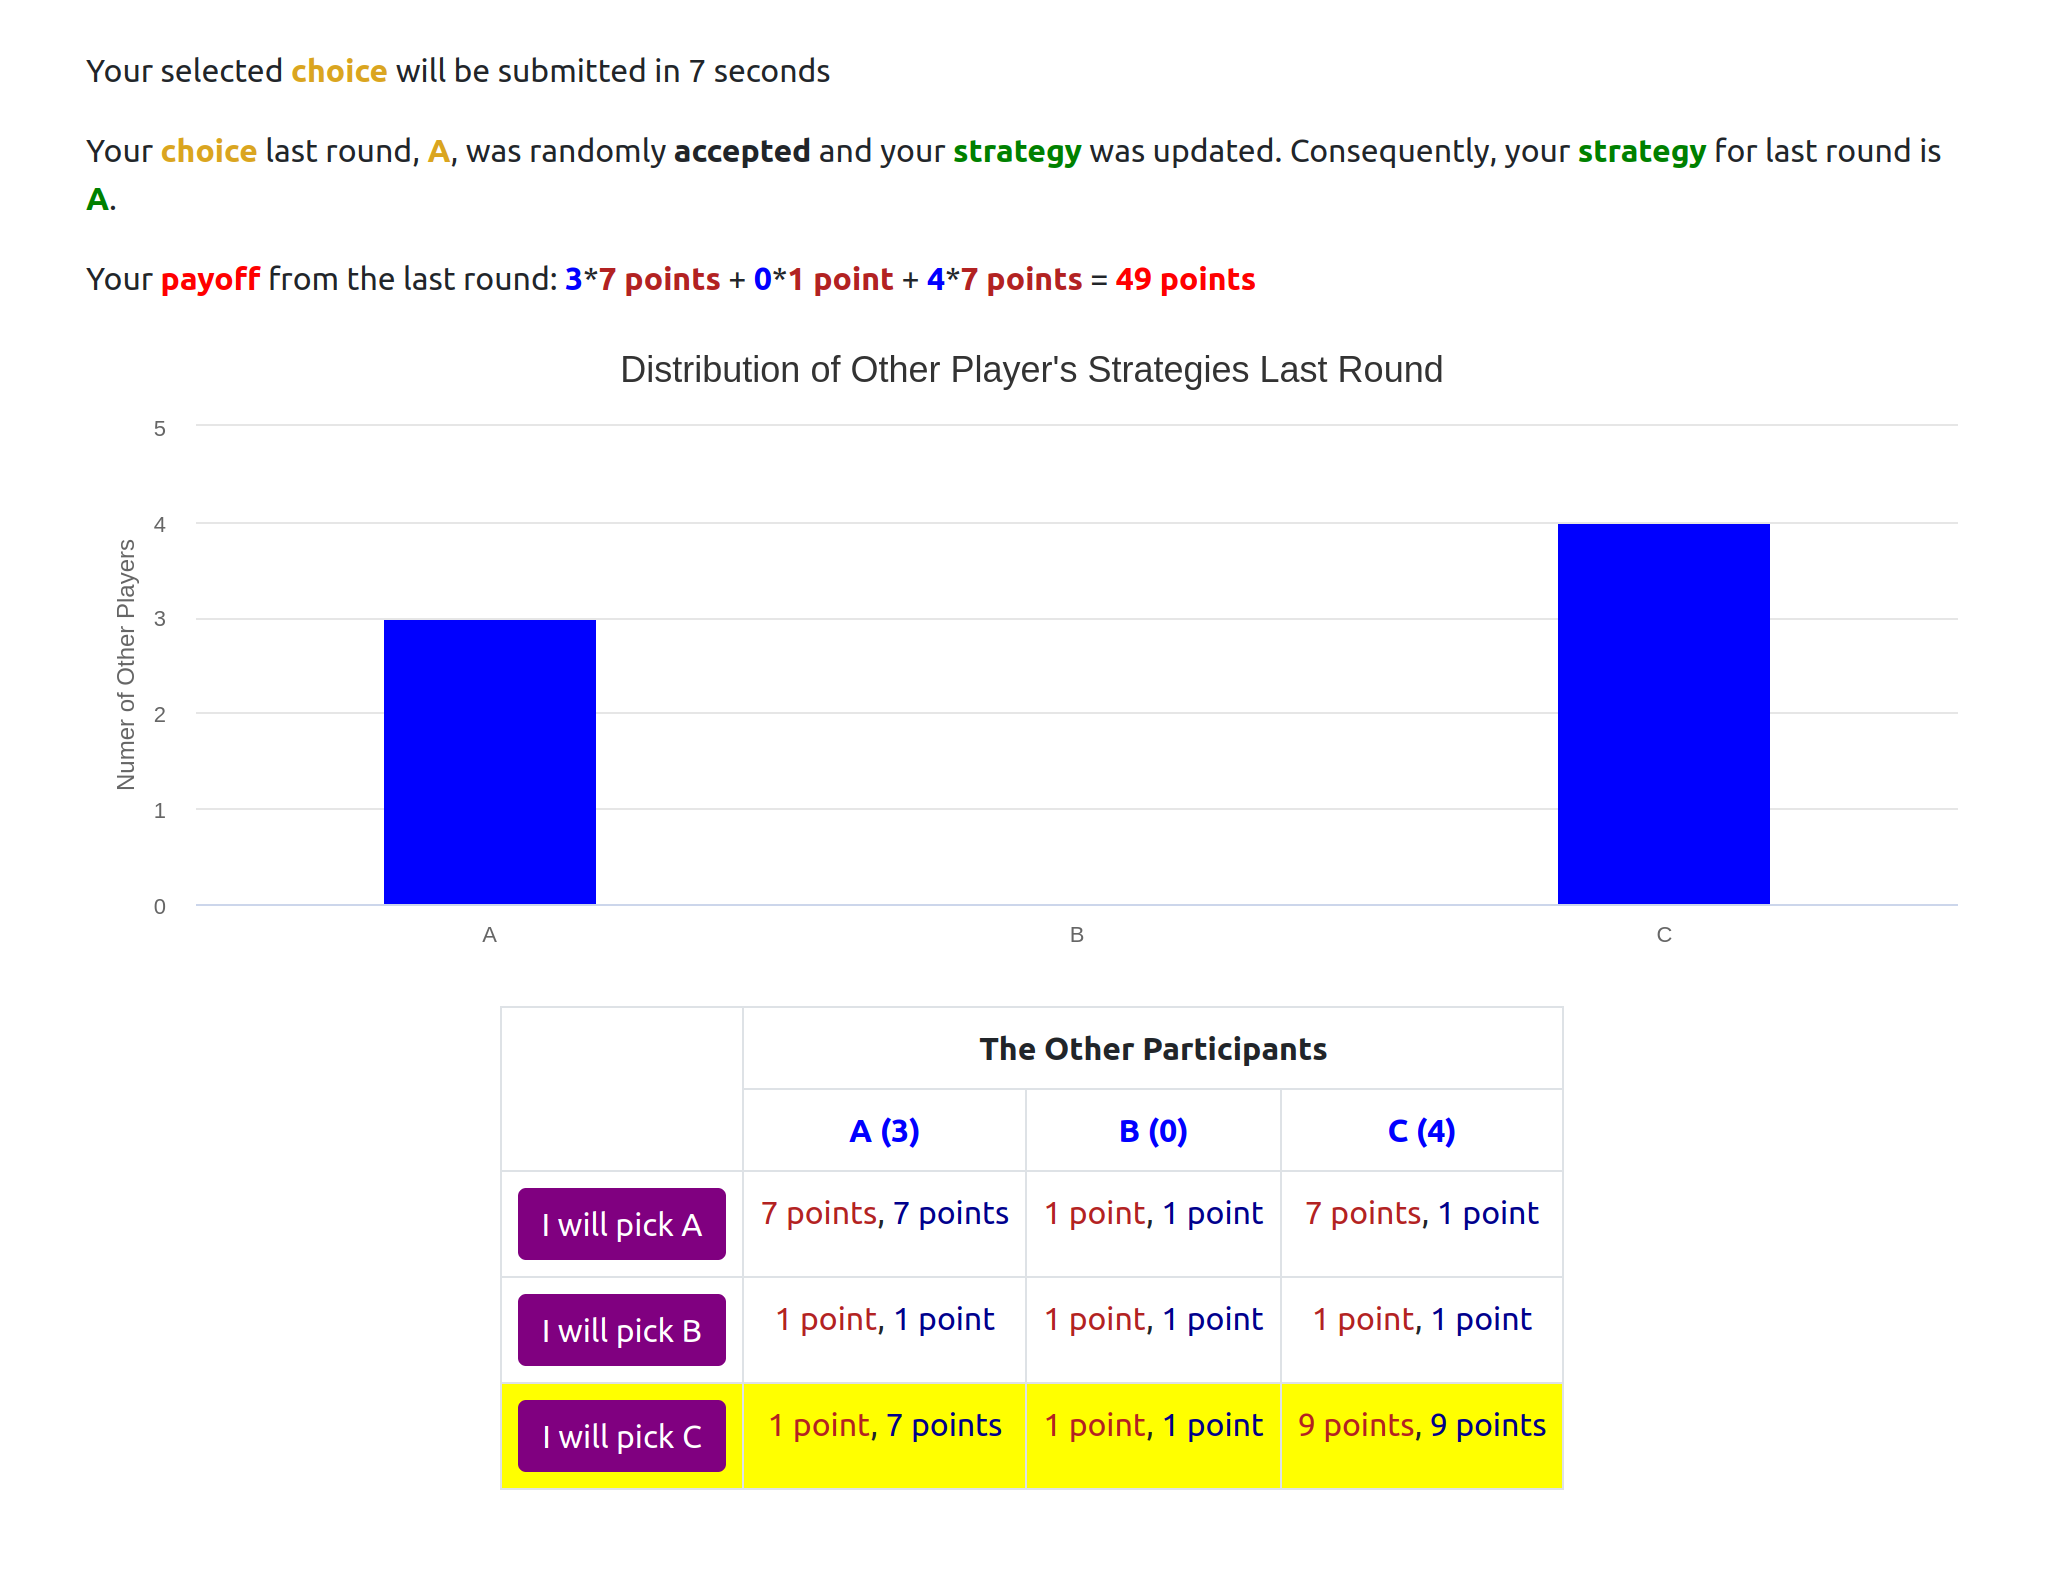
\includegraphics[width = \textwidth]{Images/Game1Choice.png}
\end{figure}

\begin{figure}[h]
\captionsetup{justification=centering}
  \caption{Experiment UI 2}
   \label{fig:UI2}
    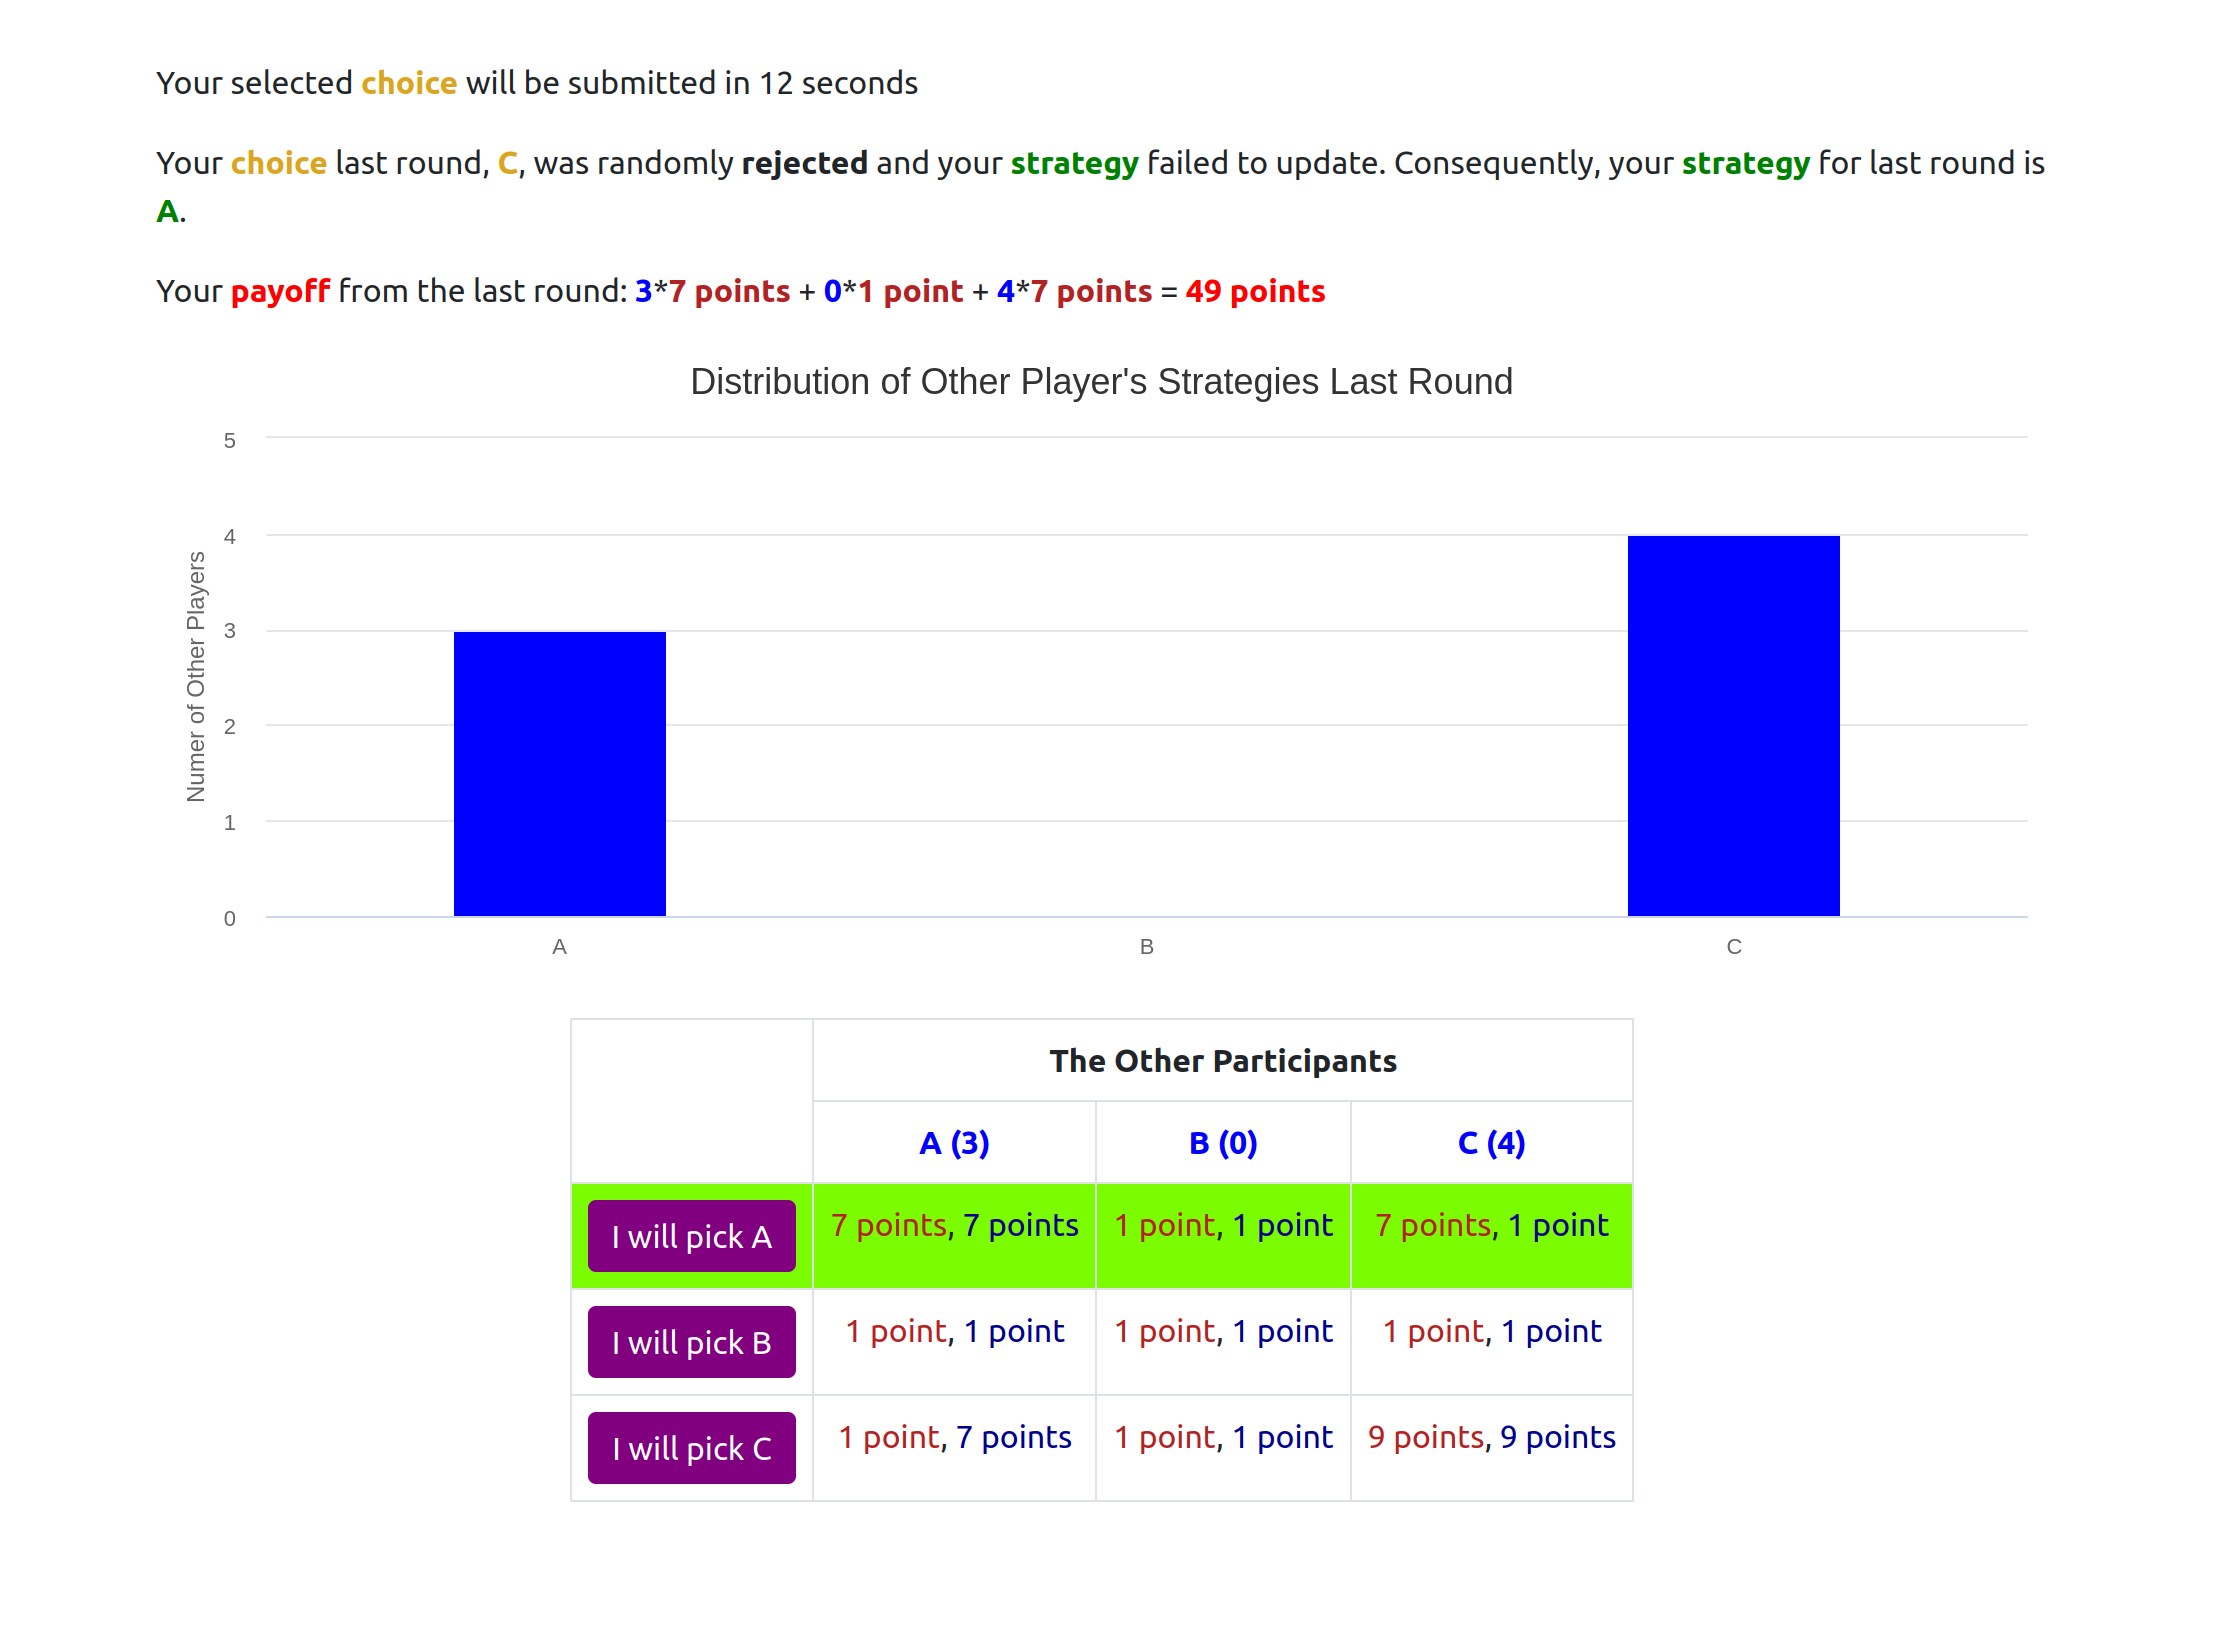
\includegraphics[width = \textwidth]{Images/Game1Reject.png}
\end{figure}



